\documentclass[11pt,a4paper]{article}
\usepackage{amsmath,amssymb,amsthm,graphicx,hyperref,booktabs,placeins}
\usepackage[margin=2.3cm]{geometry}
\newtheorem{theorem}{Theorem}
\newtheorem{proposition}[theorem]{Proposition}
\newtheorem{conjecture}[theorem]{Conjecture}
\theoremstyle{remark}\newtheorem{remark}[theorem]{Remark}
\graphicspath{{../FIGURES/}}

\title{Inner-horizon instability of regular black holes in quasi-topological gravity:\\
a Tipler-weak null singularity in $D=5$, curvature-bounded mass inflation in $D=10$,\\ and the inner-extremal exception}
\author{Project Baby Universe --- Genesis Branch\\ \small(draft for external review; not submitted)}
\date{31 October 2026}

\begin{document}
\maketitle

\begin{abstract}
Infinite towers of quasi-topological curvature corrections in $D\geq5$ make the Schwarzschild--Tangherlini singularity regular: the unique
spherically symmetric vacuum solution has a de Sitter core and an inner horizon (Bueno, Cano and Hennigar). We evolve the coupled
gravity--massless-scalar system of such a theory in double-null coordinates, using constraints derived from the first law of the reduced
action and a hybrid formulation that carries the mass function by its exact fluxes, which keeps the solution inside the domain of the
tower ($\psi<1/\alpha$). For the Hayward tower in $D=5$ a scalar pulse drives mass inflation at the Cauchy horizon: the Kretschmann
scalar grows by more than ten orders of magnitude while the area radius stays finite. Along an outgoing null ray the affine distance to
the Cauchy horizon is finite and the Tipler integral converges ($I_T=0.0327$, two resolutions agree to $0.2\%$), so the singularity is
deformationally weak; we prove that convergence of $I_T$ is equivalent to bounded total focusing of the area radius. The Kr\'olak
integral grows ($\sim410$--$520$), so its strength in Kr\'olak's sense is undetermined and the metric extension is at best $C^0$.
In $D=10$ the mass grows threefold while $\psi\alpha\to0.990$ and the curvature stays at the de Sitter-core scale through the converged
range ($v\lesssim14.5\,l$); later times are not converged. For an inner-extremal tower ($\kappa_-=0$, tuned mass) there is no mass
inflation within $v\le36\,l$ (mass $+1\%$, $Kl^4\le106$) and rays cross the inner horizon at finite advanced time. Consequences for the
continuation of the interior (``daughter'' regions) are stated precisely.
\end{abstract}

\section{Introduction}
Regular black holes generically have an inner horizon, and inner horizons are generically unstable: perturbations blueshift there and
drive mass inflation (Poisson--Israel 1990; Ori 1991). Whether a pure-gravity regularisation escapes the instability is a dynamical
question. Bueno, Cano and Hennigar showed that in $D\ge5$ an infinite tower of quasi-topological densities has the Hayward,
Bardeen-like and Dymnikova-like metrics as its unique spherically symmetric vacua [BCH, arXiv:2403.04827]; thin-shell collapse and
Oppenheimer--Snyder collapse in these theories were analysed in [arXiv:2412.02740, 2412.02742, 2505.09680], and inner-extremal
versions free of classical mass inflation were constructed for a tuned mass [Di Filippo--Kol\'a\v{r}--Kubiz\v{n}\'ak, arXiv:2404.07058].
Null thin shells cannot be used to probe the inner horizon in these theories [arXiv:2604.27980], and Frolov--Zelnikov
[arXiv:2601.01861] find significant mass inflation only for crossings close to the horizon. What has been missing is a continuous-flux,
nonlinear evolution with a characterisation of the resulting singularity. This paper provides it.

\section{Model and equations}
The metric is $ds^2=-2e^{2\sigma}du\,dv+r^2d\Omega_{D-2}^2$ and the tower enters through
$\psi=(1+2e^{-2\sigma}r_ur_v)/r^2$ and $h(\psi)$ with $\mu=r^{D-1}h(\psi)$ (Hayward: $h=\psi/(1-\alpha\psi)$; Dymnikova:
$h=-\ln(1-\alpha\psi)/\alpha$; GR: $h=\psi$). Units $l=1$, $\alpha=1$. With a minimally coupled massless scalar $\phi$:
\begin{align}
h'(\psi)\,(r_{uu}-2\sigma_ur_u)&=-r\phi_u^2,\qquad h'(\psi)\,(r_{vv}-2\sigma_vr_v)=-r\phi_v^2,\\
r_{uv}&=\tfrac{r e^{2\sigma}}{2}\Big(2\psi-(D-1)\frac{h}{h'}\Big),\qquad
\phi_{uv}=-\frac{D-2}{2r}(r_u\phi_v+r_v\phi_u),
\end{align}
with $\sigma_{uv}$ obtained symbolically from the reduced action (exact GR limit; static check $\sigma_{uv}=-ff''/8$). The mass function
obeys the first-law fluxes $\mu_u=-2r^{D-2}e^{-2\sigma}r_v\phi_u^2$, $\mu_v=-2r^{D-2}e^{-2\sigma}r_u\phi_v^2$. The \emph{hybrid} scheme
evolves $(r,\sigma,\mu,\phi)$ and recovers $\psi=h^{-1}(\mu/r^{D-1})$, so that $\psi<1/\alpha$ is automatic. An $(r,\sigma)$ formulation
drifts near the Cauchy horizon and a pure $\mu$ formulation fails at apparent horizons (both documented as failed approaches).
The static hole is reproduced to $10^{-7}$ and the scheme converges at second order.

\section{Singularity strength}
Along an outgoing null ray $u=$ const the affine parameter is $d\lambda=e^{2\sigma}dv$ and the constraint becomes
\begin{equation}
\frac{d^2r}{d\lambda^2}=-\frac{r\,\tilde R}{D-2},\qquad \tilde R\equiv\frac{(D-2)\phi_\lambda^2}{h'(\psi)}\ \ge0 ,
\end{equation}
which reduces to the Raychaudhuri equation with $\tilde R=R_{kk}$ in GR. Define the Kr\'olak and Tipler integrals
$I_K(\lambda)=\int_0^\lambda\tilde R$, $I_T(\lambda)=\int_0^\lambda d\lambda'\int_0^{\lambda'}\tilde R$.
\begin{theorem}[area control]\label{thm:area}
If $r\in[r_1,r_2]$ with $r_1>0$ on $[0,\lambda_*)$, $\lambda_*<\infty$, then
$r_1I_T(\lambda)/(D-2)\le r(0)+r_\lambda(0)\lambda-r(\lambda)\le r_2I_T(\lambda)/(D-2)$. Hence $I_T(\lambda_*)<\infty$ iff the total
focusing of $r$ is finite, and $r_\lambda(\lambda_*)$ is finite iff $I_K(\lambda_*)<\infty$.
\end{theorem}
\begin{proof}Integrate the focusing equation twice and bound $r$ between $r_1$ and $r_2$; $\tilde R\ge0$ since $h'>0$.\end{proof}

\begin{proposition}[numerical; $D=5$ Hayward, $\mu_0=10$]
After a pulse of amplitude $0.05$ (and with an additional $v^{-3}$ tail of amplitude $0.01$), along an interior outgoing ray at two
resolutions ($2000\times8000$, $4000\times16000$): $\lambda_*=1.028$--$1.036$, $r\to1.0521$ (agreement $10^{-5}$),
$I_T\to0.03263/0.03269$ (pulse) and $0.03223/0.03230$ (tail), while $I_K=413/409$ and $520/515$ at $v=26$, still growing. The
curvature grows by $6\times10^{11}$, $2\times10^{10}$ and $2\times10^{11}$ for $\psi_-\alpha=0.887,0.958,0.990$.
\end{proposition}
By Theorem~\ref{thm:area} the Cauchy horizon is a \emph{Tipler-weak null singularity}: finite affine distance, finite area radius,
finite total focusing. If $I_K$ diverges, $r_\lambda$ diverges and the metric is at best $C^0$-extendible; the continuation is then not
fixed by the field equations.

\section{$D=10$ and the inner-extremal tower}
\begin{proposition}[numerical; $D=10$ Hayward, $\mu_0=3\mu_{\rm ext}$]
Through $v\approx14.5\,l$ (resolutions $4000\times16000$ and $8000\times32000$ agree): $\mu:32.5\to102.6$, $\psi\alpha=0.9899$,
$I_K=4.77$, $I_T=0.127$, $150\le Kl^4\le400$ (the de Sitter core scale is $2D(D-1)=180$). For three masses the inner apparent horizon is
crossed at $v=8$--$14$ with curvature growth $2$--$140$. After $v\approx14.5$ the resolutions disagree (spikes to $3\times10^8$ and
$1.7\times10^5$); this regime is not resolved.
\end{proposition}
\begin{conjecture}[curvature-saturated mass inflation]
In $D=10$ the mass inflates while $\psi\to1/\alpha$ and the curvature remains at the core scale. (Supported only in the converged range.)
\end{conjecture}
\begin{proposition}[numerical; inner-extremal tower]
For $f$ with a triple root at $r_-^2=1.5$ and a simple root at $r_+^2=9$ ($\mu=16$, $\kappa_-=0$), the same pulse gives, at two
resolutions, $\mu\to16.17$ ($+1\%$), $Kl^4\le106$, and the interior ray crosses $r_-$ at $v=27.36/27.38$.
\end{proposition}
In the Ori model the inner mass function scales as $e^{\kappa_-v}$ times the tails; for $\kappa_-=0$ and tails $v^{-p}$, $p>1$, it stays
bounded, independently of the angular mode. Two caveats: the property is fine-tuned (accretion detunes it; the run's own $1\%$ mass gain
splits the triple root and restores a small $\kappa_-$), and an inner-horizon instability remains semiclassically
[McMaken, arXiv:2303.03562].

\begin{figure}[t]\centering
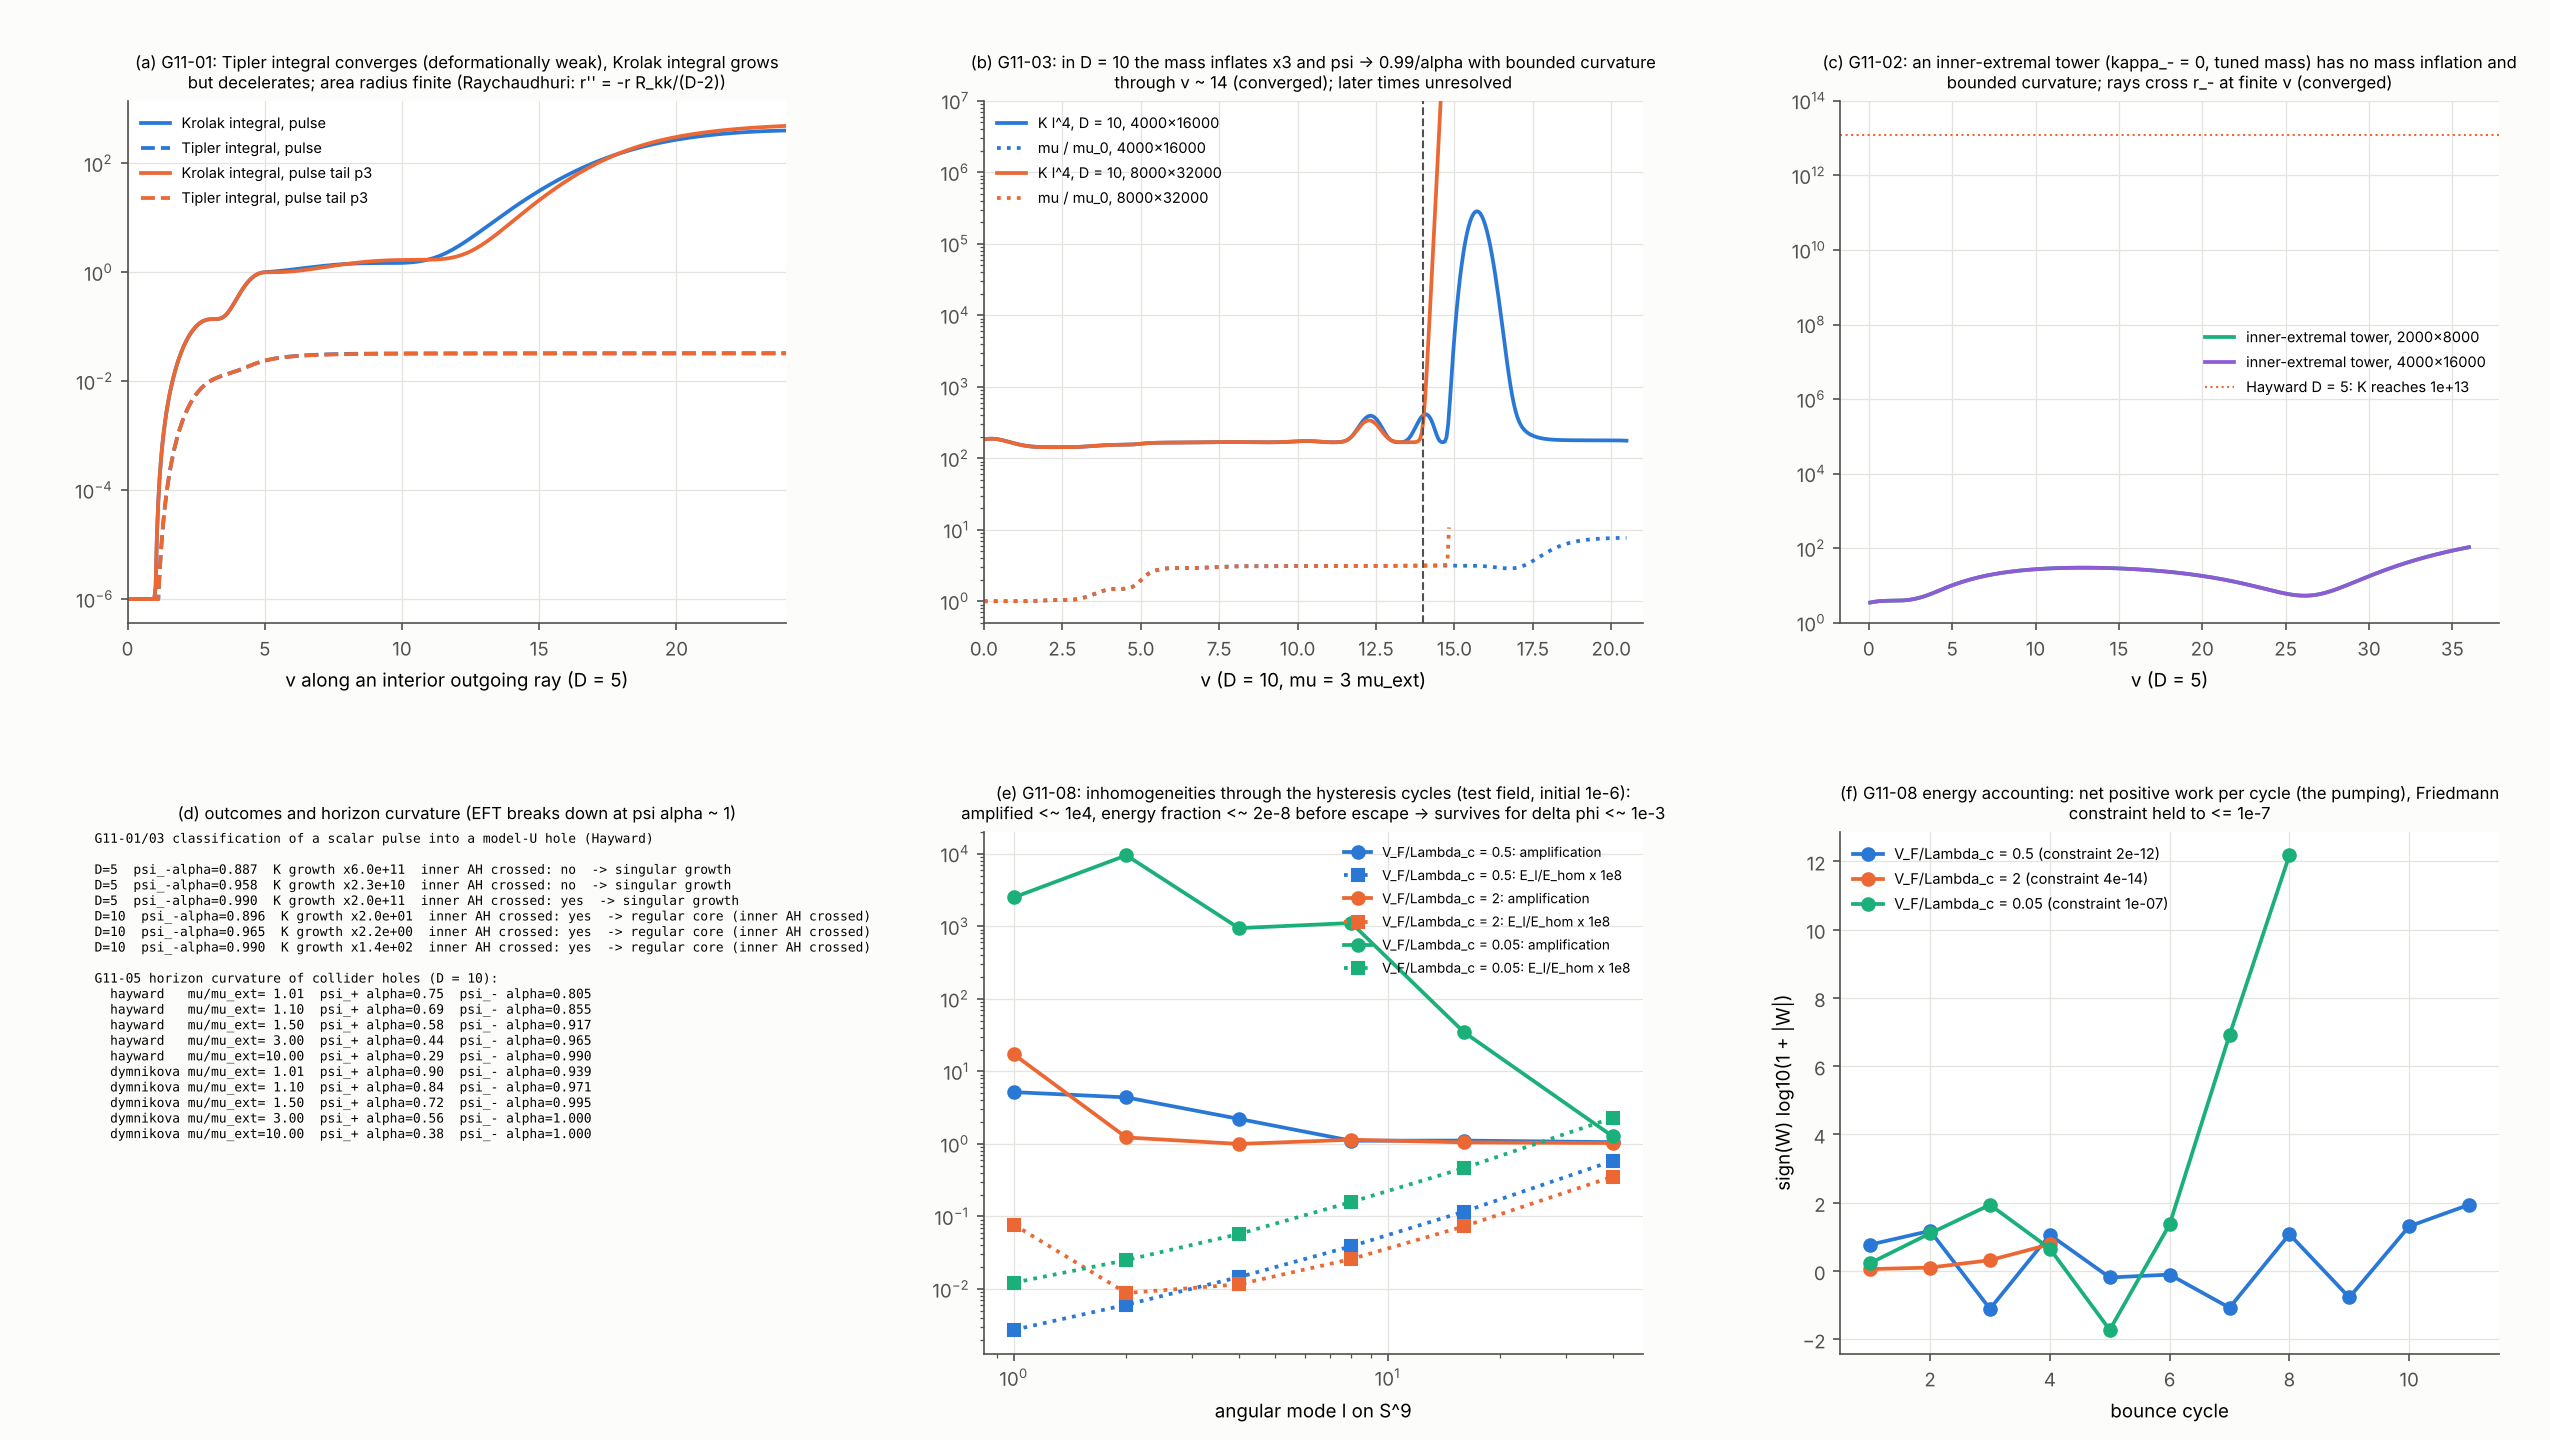
\includegraphics[width=\textwidth]{round11_physics.png}
\caption{(a) Kr\'olak and Tipler integrals along an interior ray ($D=5$). (b) $D=10$: curvature and mass, two resolutions; the dashed line
marks the end of the converged range. (c) Inner-extremal tower. (d) Classification and horizon curvature of collider holes.
(e,f) Hysteresis track (not discussed in this paper).}\end{figure}

\begin{figure}[t]\centering
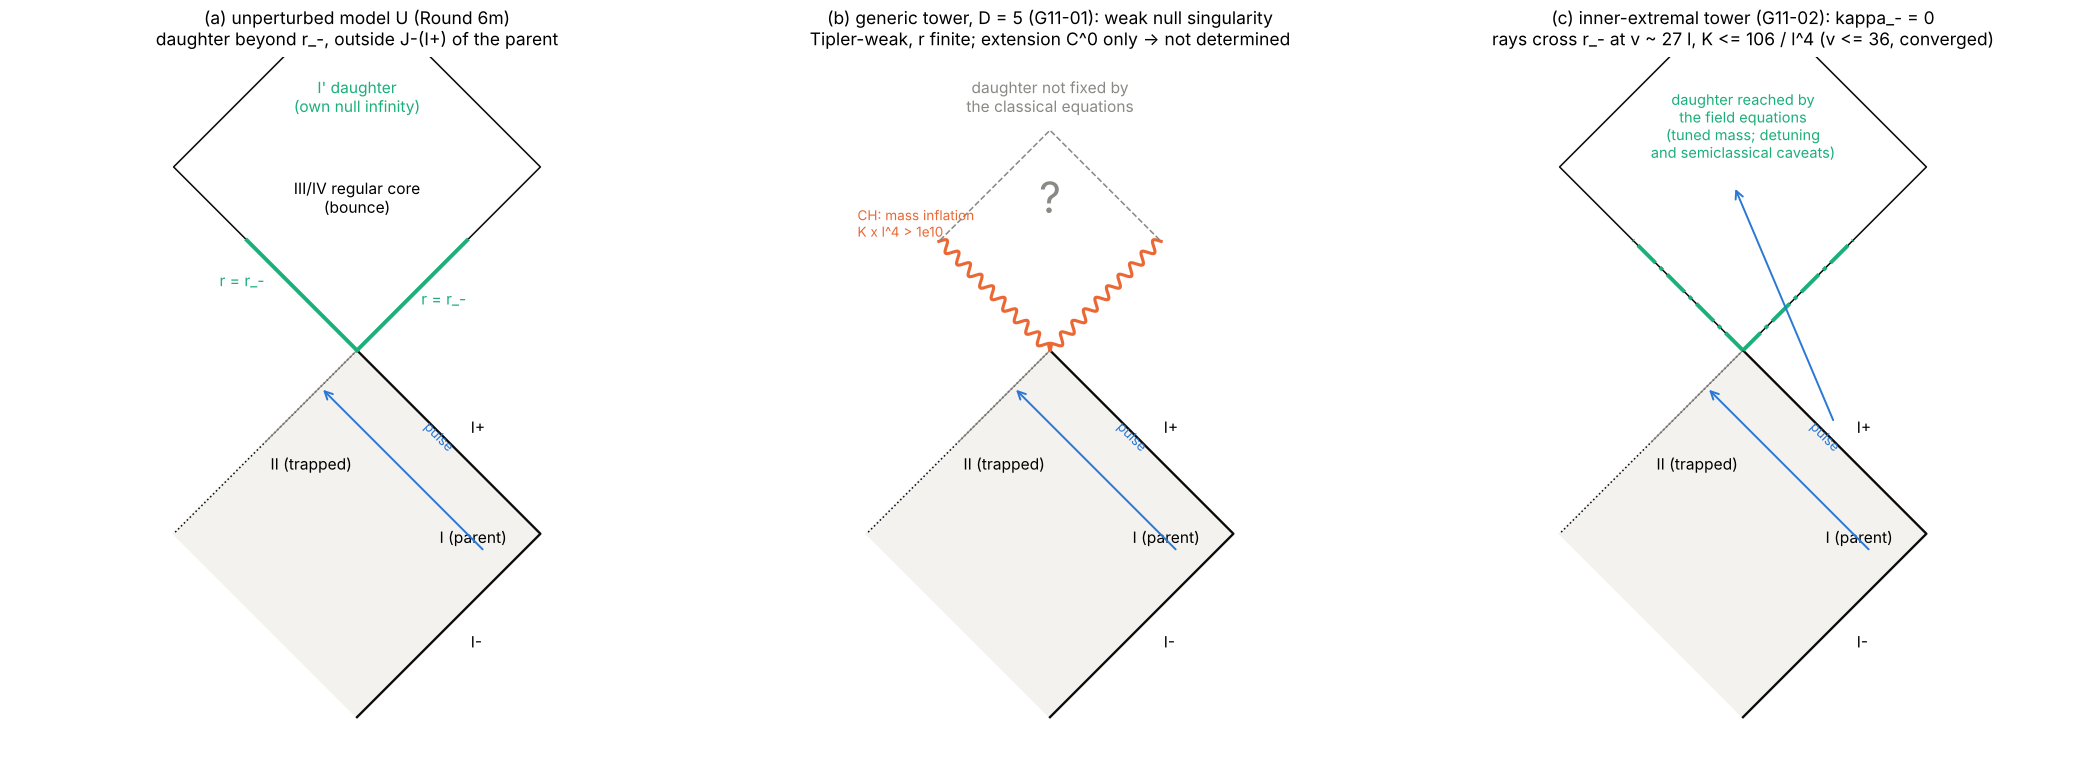
\includegraphics[width=\textwidth]{round11_causal.png}
\caption{Schematic conformal diagrams: unperturbed geometry; generic $D=5$ evolution with a weak null singularity at the Cauchy horizon;
inner-extremal tower.}\end{figure}

\section{Discussion}
\begin{itemize}
\item The pure-gravity regularisation removes the central singularity of the static solution but not the inner-horizon instability:
in $D=5$ the dynamical interior ends at a weak null singularity of Ori type. Regular ``daughter'' regions beyond the inner horizon of
the static solution are therefore not a prediction of the classical dynamics for generic data.
\item $D=10$ behaves differently over the converged range; whether this persists requires a compactified-$v$ code with mesh refinement.
\item The inner-extremal family is the only case in which the field equations carry the solution across $r_-$; it is non-generic.
\item Limitations: spherical symmetry; a single minimally coupled scalar; no semiclassical source; well-posedness of the full tower
off spherical symmetry is open (the tower contains Gauss--Bonnet, which loses hyperbolicity near small holes, Reall--Tanahashi--Way
arXiv:1406.3379); horizon values $\psi_+\alpha=0.3$--$0.9$ for collider-mass holes put the tower outside any EFT truncation.
\end{itemize}

\section*{Reproducibility}
All results are produced by \texttt{CODE/scripts/round11\_physics.py} (modules \texttt{strength11}, \texttt{stable11},
\texttt{doublenull10}); data in \texttt{DATA/round11\_physics.json}; tests in \texttt{CODE/tests/test\_round11.py}. The originality
audit is \texttt{ROUND11/publications/ORIGINALITY\_AUDIT.md}.

\section*{References}
\small
Bueno, Cano, Hennigar, PLB 861 (2025), arXiv:2403.04827.
Bueno, Cano, Hennigar, Murcia, PRD 111, 104009 (2025), arXiv:2412.02740; PRL 134, 181401 (2025), arXiv:2412.02742.
Bueno, Cano, Hennigar, Murcia, Vicente-Cano, arXiv:2505.09680.
Di Filippo, Kol\'a\v{r}, Kubiz\v{n}\'ak, PRD 111, L041505 (2025), arXiv:2404.07058.
Di Filippo, Kubiz\v{n}\'ak, Srinivasan, PRD 114, 044061 (2026), arXiv:2604.27980.
Frolov, Zelnikov, PRD 113, 084007 (2026), arXiv:2601.01861.
Carballo-Rubio, Di Filippo, Liberati, Pacilio, Visser, JHEP 09 (2022) 118, arXiv:2205.13556.
McMaken, PRD 107, 125023 (2023), arXiv:2303.03562.
Poisson, Israel, PRD 41, 1796 (1990). Ori, PRL 67, 789 (1991).
Reall, Tanahashi, Way, arXiv:1406.3379. Papallo, Reall, arXiv:1705.04370.
Konoplya, Zhidenko, PRD 109, 104005 (2024), arXiv:2403.07848.
\end{document}
